%!TEX root=paper.tex
\section{Evaluation}
\label{sec:evaluation}

In this chapter, we will investigate the scalability of Gilbert and its performance compared to well known hand-tuned ML algorithms.
We show that Gilbert is not only easily usable in terms of programming but also produces results with decent performance.

\textbf{Experimental Setup}. For our evaluation, we use a Google compute engine cluster with $8$ machines of type \code{n1-standard-16}.
Each machine is equipped with $60$ gigabytes of main memory and has $16$ virtual CPUs. 
The Spark execution engine runs on Apache Spark-2.0.0~\cite{spark}.
For the Flink execution engine, we use Apache Flink-1.1.2~\cite{flink}. 
As underlying distributed file system both systems use Apache Hadoop-2.7.3~\cite{hadoop:2008a}.

\subsection{Scalability}

The scalability evaluation investigates how Gilbert behaves under increasing work loads and how well it can exploit varying cluster sizes.
As we have implemented Gilbert to provide a scalable linear algebra environment, it is important that it can process data sizes exceeding the main memory of a single machine.

\textbf{Matrix Multiplication}. 
As a first benchmark, we choose the matrix multiplication $A\times B$ with $A,B \in \mathbb{R}^{n\times n}$ and $n$ being the dimensionality. 
The matrix multiplication operation is demanding, both in CPU load as well as network I/O as it requires two network shuffles. 
The matrices $A$ and $B$ are sparse matrices with uniformly distributed non-zero cells. 
They are randomly generated prior to the matrix multiplication with a sparsity of $0.001$. 
As baseline, we run the same matrix multiplication on a single machine of the cluster using Gilbert's local execution engine. 
The Flink and Spark execution engines are both started with 48 gigabytes of main memory for their task managers and they distribute the work equally among all worker nodes. 
In the first experiment, we fixed the block sizes to $500 \times 500$ and set the number of cores to $64$. 
We then increased the dimensionality $n$ of $A$ and $B$ to observe the runtime behavior. 
The resulting execution times for the local, Flink and Spark execution engines are shown in \cref{fig:mmLoadRuntime}. 
In the second experiment, we investigate the scaling behavior of Gilbert with respect to the cluster size. 
In order to observe the communication costs, we keep the work load per core constant while increasing the number of cores. 
For this experiment we vary the number of cores from $1$ to $128$ and scale $n$ such that $n^3/\#cores$ is constant. 
We started with $n=5000$ for a single core and reached $n=25000$ on $128$ cores. 
The results of the experiment are shown in \cref{fig:mmNodesRuntime}. 

On a single machine, we are able to execute the matrix multiplication for dimensionalities up to $n=10000$ in a reasonable time. 
We can see that the local execution performs better for dimensionalities $n \le 2500$. 
That is expected since the matrix still fits completely in the main memory of a single machine and the distributed execution adds communication overhead and job start up latency.
For matrices with $n>2500$, Spark and Flink start to calculate the matrix multiplication faster than the local executor. 
We also see that Gilbert can handle matrix sizes which scale far beyond what a single machine can handle. 

The results depicted in \cref{fig:mmNodesRuntime} indicate for both execution engines decent scale-out behavior.
For Spark we observe an almost horizontal line for number of cores $\le 32$.
For larger number of cores, the scaling degrades which is probably caused by spilling.
The same applies to Flink.
However, we can observe that the system has to start spilling data earlier.
Thus, Flink's scale-out behaviour is not as good as Spark's with respect to matrix multiplication.

\begin{figure}[htbp]
	\centering
	\begin{subfigure}{\dualpgfwidth}
		\begin{tikzpicture}
			\begin{loglogaxis}[
				xlabel={Dimensionality $n$},
				ylabel={Execution time $t$ in s},
				width=\dualpgfwidth,
				height=.78\dualpgfwidth,
				legend entries={Local, Spark, Flink},
				legend pos=north west,
				font=\footnotesize
			]
			\addplot[
				color=blue,
				mark=x,
			] table[
				x=RowsA,
				y=Time,
			]
			{data/matrixMult/matrixMultLoadReference};
			\addplot[
				color=red,
				mark=o,
			] table[
				x=RowsA,
				y=Time,
			]
			{data/matrixMult/matrixMultLoadSpark};
			\addplot[
				color=teal,
				mark=triangle,
			] table[
				x=RowsA,
				y=Time,
			]
			{data/matrixMult/matrixMultLoadFlink};
			\end{loglogaxis}
		\end{tikzpicture}
		\caption{}
		\label{fig:mmLoadRuntime}
	\end{subfigure}
	\begin{subfigure}{\dualpgfwidth}
		\begin{tikzpicture}
			\begin{semilogxaxis}[
				xlabel={Number of cores},
				ylabel={Execution time $t$ in s},
				legend pos=north west,
				legend entries={Spark, Flink},
				ymin=0.0,
				ymax=2000,
				width=\dualpgfwidth,
				height=.78\dualpgfwidth,
				font=\footnotesize
			]
			\addplot[
				color=red,
				mark=o,
			] table[
				x=Parallelism,
				y=Time,
			]
			{data/matrixMult/matrixMultScalabilitySpark};
			\addplot[
				color=teal,
				mark=triangle,
			] table[
				x=Parallelism,
				y=Time,
			]
			{data/matrixMult/matrixMultScalabilityFlink};
			\end{semilogxaxis}
		\end{tikzpicture}
		\caption{}
		\label{fig:mmNodesRuntime}
	\end{subfigure}
	\caption{Scalability of matrix multiplication. \subref{fig:mmLoadRuntime} Execution time of matrix multiplication depending on the data size. \subref{fig:mmNodesRuntime} Execution time of matrix multiplication depending on the cluster size with constant work load per core.}
	\label{fig:mmScalability}
\end{figure}

\textbf{Gaussian Non-negative Matrix Factorization}. As second benchmark, we choose the Gaussian non-negative matrix factorization (GNMF) algorithm~\cite{seung:anips2001a}.
GNMF finds for a given matrix $V \in \mathbb{R}^{d\times w}$ a factorization $W \in \mathbb{R}^{d\times t}$ and $H \in \mathbb{R}^{t\times w}$ such that $V\approx W H$ holds true.
For our evaluation, we calculate one step of the GNMF algorithm.
We set $t=10$, $w=100000$ and vary the number of rows $d$ of $V$.
The matrix $V\in\mathbb{R}^{d\times 100000}$ is a sparse matrix whose sparsity is set to $0.001$.
The non-zero cells of $V$ are uniformly distributed.
As baseline, we run the GNMF on a single machine of the cluster using the local execution engine.
Like for the matrix multiplication benchmark, the task manager of Spark and Flink are started with 48 gigabytes of memory.
In the first experiment we fix the number of cores to $64$.
We start with $d=500$ and increase the number of rows of $V$ to $150000$.
The block size of Gilbert is set to $500 \times 500$.
In order to compare the results with the optimized GNMF MapReduce implementation proposed in~\cite{liu:2010a}, we re-implemented the algorithm using  Spark and Flink.
This hand-tuned implementation, henceforth denoted as HT-GNMF (HT in the graphs), is also executed on $64$ cores.
The execution times of HT-GNMF and Gilbert's GNMF are shown in \cref{fig:nmfLoadRuntime}.
In the second experiment of the GNMF benchmark, we analyze how Gilbert scales-out when increasing the cluster size while keeping the work load for each core constant.
We vary the cluster size from $1$ core to $64$ cores and scale the number of documents $d$ accordingly.
Initially we start with $1000$ documents and, consequently, calculate the matrix factorization for $64000$ documents on $64$ cores.
The results of this experiment are shown in \cref{fig:nmfNodesRuntime}.

\begin{figure}[htbp]
	\centering
	\begin{subfigure}{\dualpgfwidth}
		\begin{tikzpicture}
			\begin{loglogaxis}[
				xlabel={Number of rows of matrix $V$},
				ylabel={Execution time $t$ in s},
				width=\dualpgfwidth,
				height=.78\dualpgfwidth,
				legend pos=north west,
				legend columns=2,
				legend entries={Local, Spark, Flink, HT Spark, HT Flink},
				ymax=800,
				font=\footnotesize
			]
			\addplot[
				color=blue,
				mark=x,
			] table[
				x=Rows,
				y=Time,
			]
			{data/nnmfStep/nnmfStepLoadReference};
			
			\addplot[
				color=red,
				mark=o,
			] table[
				x=Rows,
				y=Time,
			]
			{data/nnmfStep/nnmfStepLoadSpark};
			
			\addplot[
				color=teal,
				mark=triangle,
			]table[
				x=Rows,
				y=Time,
			]
			{data/nnmfStep/nnmfStepLoadFlink};
			\addplot[
				color=black,
				mark=diamond,
			]table[
				x=rowsV,
				y=time,
			]
			{data/nnmfStep/gnmfStepBenchLoadSpark};
			\addplot[
				color=magenta,
				mark=square,
			]table[
				x=rowsV,
				y=time,
			]
			{data/nnmfStep/gnmfStepBenchLoadFlink};
			\end{loglogaxis}
		\end{tikzpicture}
		\caption{}
		\label{fig:nmfLoadRuntime}
	\end{subfigure}
	\begin{subfigure}{\dualpgfwidth}
		\begin{tikzpicture}
			\begin{semilogxaxis}[
				xlabel={Number of rows of matrix $V$},
				ylabel={Speedup of HT over Gilbert},
				width=\dualpgfwidth,
				height=.78\dualpgfwidth,
				ymin=0,
				ymax=2.5,
				legend entries={Spark,Flink},
				legend pos=north west,
				font=\footnotesize
			]
			\addplot[
				color=red,
				mark=o,
			] table[
				x=Rows,
				y=Speedup,
			]
			{data/nnmfStep/gnmfStepSpeedupSpark};

			\addplot[
				color=teal,
				mark=diamond,
			] table[
				x=Rows,
				y=Speedup,
			]
			{data/nnmfStep/gnmfStepSpeedupFlink};
			\end{semilogxaxis}
		\end{tikzpicture}
		\caption{}
		\label{fig:gnmfSpeedup}
	\end{subfigure}
	\begin{subfigure}{\dualpgfwidth}
		\begin{tikzpicture}
			\begin{semilogxaxis}[
				xlabel={Number of cores},
				ylabel={Execution time $t$ in s},
				xmax=101,
				ymin=0,
				ymax=60,
				legend entries={Spark, Flink},
				legend pos=north west,
				width=\dualpgfwidth,
				height=.7\dualpgfwidth,
				font=\footnotesize
			]
			\addplot[
				color=red,
				mark=o,
			] table[
				x=Parallelism,
				y=Time,
			]
			{data/nnmfStep/nnmfStepScalabilitySpark};

			\addplot[
				color=teal,
				mark=diamond,
			] table[
				x=Parallelism,
				y=Time,
			]
			{data/nnmfStep/nnmfStepScalabilityFlink};
			\end{semilogxaxis}
		\end{tikzpicture}
		\caption{}
		\label{fig:nmfNodesRuntime}
	\end{subfigure}
	\caption{Scalability of GNMF. \subref{fig:nmfLoadRuntime} Execution time of one GNMF step depending on the data size. \subref{fig:gnmfSpeedup} Speedup of HT-GNMF over Gilbert's GNMF using Spark and Flink. \subref{fig:nmfNodesRuntime} Execution time of one GNMF step depending on the cluster size with constant work load per core.}
	\label{fig:nmfBenchmark}
\end{figure}

The local executor is applied to sizes of $d$ ranging from $500$ to $3000$ rows.
Surprisingly, the local execution is outperformed by the distributed engines.
This fact indicates that the network communication costs are not decisive.
The distributed systems can also be used for data sizes which can no longer be handled by a single machine.
Both distributed execution engines scale well and achieve almost identical results as the hand tuned implementations.
The speedup of the HT-GNMF variants compared to GNMF on Spark's and Flink's executor is shown in \cref{fig:gnmfSpeedup}.
In the case of Flink, the HT-GNMF variant runs at most $1.78$ times faster than Gilbert's GNMF implementation for large data sets.
For Spark, we can only observe a maximum speedup of $1.35$.
This result underlines Gilbert's good performance.

Furthermore, the development with Gilbert was considerably easier.
One GNMF step can be programmed in five lines of Gilbert code, whereas we needed $28$ lines of Scala code for Spark's HT-GNMF and $70$ lines of Scala code for Flink's HT-GNMF.
Not only did we have to know how to program Spark and Flink, but it also took us quite some time to verify the correct functioning of both implementations.
The verification was made significantly more difficult and time-consuming due to a programming bug we introduced.
The debugging process showed us quite plainly how tedious the development process even with systems like Spark and Flink can be.
Thus, the productivity increase gained by using a high-level declarative programming language for linear algebra must not be neglected and compensates for the slight performance loss.
\cite{alvaro:2010a} made similar observations while developing a declarative programming language for distributed systems programming.
The scale-out behavior of the Flink and Spark execution engines \cref{fig:nmfNodesRuntime} both show good results for $\#cores$ up to $64$.
The runtime on Spark with $64$ cores is only $1.26$ times slower than the runtime on a single core with the same work load per core.
For Flink we observe a slowdown of $2.38$ when running on $64$ cores.

\subsection{PageRank}

In this section, we want to investigate how well the PageRank algorithm~\cite{page:1999a} implemented in Gilbert performs compared to a specialized implementation (denoted as SP in the figures).
We expect that the Gilbert runtime adds some overhead.
Furthermore, the high-level linear algebra abstraction of Gilbert might make it difficult to exploit certain properties to speed up the processing.
We first execute PageRank directly in Gilbert, given the Gilbert code in \cref{lst:gilbertPageRank}, and then run them directly on Flink and Spark.
In contrast to Gilbert, the direct implementation requires a deep understanding of the underlying runtime system.
Furthermore, the distributed implementation is far from trivial compared to the linear algebra representation of the original problem.
\begin{listing}[htbp]
	\begin{lstlisting}[language=Matlab,
		commentstyle=\color{black},
		  stringstyle=\color{black},
		  keywordstyle=\color{black}\bfseries,
		  morekeywords={ones, fixpoint},
		  xleftmargin=.0\textwidth,
		  basicstyle=\footnotesize]
% load adjacency matrix
A = load();
maxIterations = 10;
d = sum(A, 2); % outdegree per vertex
% create the column-stochastic transition matrix
T = (diag(1 ./ d) * A)'; 
r_0 = ones(numVertices, 1) / numVertices; % initialize the ranks
e = ones(numVertices, 1) / numVertices;
% PageRank calculation
fixpoint(r_0, @(r) .85 * T * r + .15 * e, maxIterations)
	\end{lstlisting}
	\caption{Gilbert PageRank implementation.}
	\label{lst:gilbertPageRank}
\end{listing}
The specialized Spark and Flink implementation of PageRank works as follows.
The Page\-Rank vector is represented by a set of tuples $(w_i, r_i)$ with $w_i$ denoting the web site $i$ and $r_i$ being its rank.
The adjacency matrix is stored row-wise as a set of tuples $(w_i, A_i)$ with $w_i$ denoting the web site $i$ and $A_i$ being its adjacency list.
For the adjacency list $A_i$, it holds that $w_j \in A_i$ if and only if there exists a link from web site $i$ to $j$.
The next PageRank vector is calculated as follows.
The PageRank $r_i$ of web site $i$ is joined with its adjacency list $A_i$.
For each outgoing link $w_j \in A_i$ a new tuple $(w_j, 0.85r_i/\left|A_i\right|)$ with the rank of $i$ being divided by the number of outgoing links is created.
In order to incorporate the random jump behavior to any available web site, a tuple $(w_i, 0.15/|w|)$, with $|w|$ being the number of all web sites, is generated for each web site $i$.
In order to compute the next PageRank vector, all newly generated tuples are grouped according to their ID and summed up.
These steps constitute a single PageRank iteration whose data flow plan is depicted in \cref{fig:pageRankDataFlow}.
\begin{figure}[htbp]
	\centering
	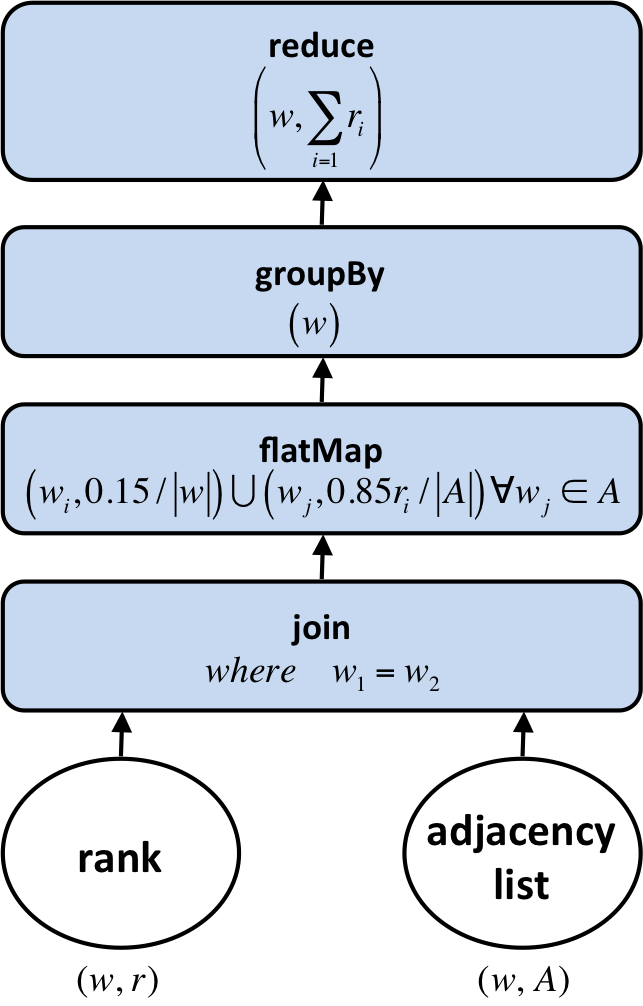
\includegraphics[width=.275\linewidth]{images/pageRankStep.png}
	\caption{Data flow of one iteration of the PageRank algorithm for Spark and Flink.}
	\label{fig:pageRankDataFlow}
\end{figure}
\textbf{Experiment}. For comparison, $10$ steps of the PageRank algorithm for varying sizes of the adjacency matrix $A$ are calculated.
The randomly generated adjacency matrix $A$ is a sparse matrix of size $n \times n$ with a sparsity of $0.001$.
The computation is executed on $64$ cores with a block size of $500 \times 500$.
The execution times are depicted in \cref{fig:pageRankResults}.
\begin{figure}[htbp]
	\centering
	\begin{subfigure}[h]{\dualpgfwidth}
		\begin{tikzpicture}
			\begin{loglogaxis}[
				xlabel={Number of vertices $n$},
				ylabel={Execution time $t$ in s},
				xmax=250000,
				ymax=50000,
				legend pos=north west,
				legend entries={Spark, Flink, SP Flink, SP Spark},
				width=\dualpgfwidth,
				height=.78\dualpgfwidth,
				font=\footnotesize
			]
			
			\addplot[blue,
				mark=x,
			] table[
				x=NumVertices,
				y=Time,
			]
			{data/pagerank/pagerankLoadSpark};

			\addplot[red,
				mark=o,
			] table[
				x=NumVertices,
				y=Time,
			]
			{data/pagerank/pagerankLoadFlink};

			\addplot[teal,
				mark=diamond,
			] table[
				x=rows,
				y=time,
			]
			{data/pagerank/pagerankBenchLoadFlink};

			\addplot[black,
				mark=triangle,
			] table[
				x=rows,
				y=time,
			]
			{data/pagerank/pagerankBenchLoadSpark};
			\end{loglogaxis}
		\end{tikzpicture}
		\caption{}
		\label{fig:pageRankResults}
	\end{subfigure}
	\begin{subfigure}[h]{\dualpgfwidth}
		\begin{tikzpicture}
			\begin{semilogxaxis}[
				xlabel={Number of vertices $n$},
				ylabel={Speedup},
				legend pos=north west,
				legend entries={SP Spark, SP Flink},
				width=\dualpgfwidth,
				height=.78\dualpgfwidth,
				font=\footnotesize
			]
			
			\addplot[blue,
				mark=x,
			] table[
				x=NumVertices,
				y=Speedup,
			]
			{data/pagerank/pagerankSpeedupSpark};

			\addplot[red,
				mark=o,
			] table[
				x=NumVertices,
				y=Speedup,
			]
			{data/pagerank/pagerankSpeedupFlink};
			\end{semilogxaxis}
		\end{tikzpicture}
		\caption{}
		\label{fig:pageRankSpeedup}
	\end{subfigure}
	\caption{Comparison of Gilbert's PageRank implementation with specialized algorithms on Spark and Flink. \subref{fig:pageRankResults} Execution time of $10$ steps of the PageRank algorithm depending on the adjacency matrix's size. \subref{fig:pageRankSpeedup} Speedup of specialized algorithms with respect to Gilbert's implementations.}
	\label{fig:pageRankEvaluation}
\end{figure}
The graphs in \cref{fig:pageRankResults} show that the specialized PageRank algorithm runs faster than Gilbert's versions of PageRank.
Furthermore, the specialized algorithms show a better scalability.
The speedup of the specialized algorithms with respect to Gilbert's implementations for this experiment is shown in \cref{fig:pageRankSpeedup}.
For $n\le 50000$, the hand-tuned algorithms running on Spark and Flink show a similar speedup.
The Flink and Spark version achieve a speedup of approximately $13$ and $12$ for $n=50000$, respectively.
However, for $n = 100000$ we can observe a speedup of $76$ for the Flink specialized implementation whereas Spark reaches a speedup of $14$.
Gilbert's performance degradation with Flink is likley caused by earlier data spilling.

The performance difference between the specialized algorithm and Gilbert's version can be explained by considering the different execution plans.
As shown in \cref{fig:pageRankDataFlow}, each iteration of the specialized PageRank algorithm comprises one join, one group reduce and one flat map operation.
In contrast, each iteration of Gilbert's PageRank implementation requires two cross, two join and one reduce operation.
Thus, it can be clearly seen that Gilbert's high-level linear algebra representation adds three additional operations, with one of them being highly expensive.
Therefore, it is not surprising that the specialized PageRank algorithm performs better.